\chapter{РАЗРАБОТКА ПРОГРАММНОГО ИНТЕРФЕЙСА}

Сначала в данной главе производится поверхностный обзор интерфейса прикладного программирования робота. Подробно рассматриваться данный компонент не будет в связи с тем, что все управление роботом в дальнейшем будет производиться через методы классов, предоставляемых симулятором Webots. Взаимодействие с интерфейсом DARwIn Framework будет происходить только при компиляции модуля для интерпретации непоследственно на самом роботе. Это связано с тем, что вызовы методов классов Webots для управления моторами на физической модели робота имеют существенные задержки во времени, которые не позволяют роботу совершать плавные и непрерывные движения.

Так же кратко будет рассмотрен интерфейс управления приводами одного из самых распространенных гуманоидных роботов Nao. Этот анализ будет произведен для получения представления о имеющихся аналогах систем управления: их плюсах и недостатках.

Далее, исходя из ранее полученных знаний, будет разработан интерфейс класса для языка программирования C++. Другие популярные языки высокого, такие как Java и Python, были исключены из-за их низкой производительности. Для поддержки данных языков в реализованного модуля управления можно воспользоваться инструментом связывания программ и библиотек, написанных на языке C и C++, с интерпретируемыми (Tcl, Perl, Python, Ruby, PHP) или компилируемыми (Java, C\#, Scheme, OCaml) языками - SWIG.


\section{Анализ DARwIn Framework}

В данном разделе будет произведет поверхностный обзор системы управления роботом, предоставляемого разработчиками платформы. Подробной документации о библиотеке производитель не распространяет.

Исходный код фреймфорка, написанного на языке C/C++, для платформы DARwIn-OP можно получить из репозитория проекта на сайте SourceForge. Исходный код распространяется под открытой лицензией. Так же используемые в данной работе классы доступны в пакете симуляции Webots в каталоге с модулями для данного робота. Симуляционная среда будет подробнее рассматриваться в следующем разделе.

Ниже приведена диаграмма классов (Рис. \ref{im:1_framework_class_diagram}), доступная в официальной документации. На данной диаграмме отображены все основные классы, которые используются при взаимодействии с роботом. % TODO Ссылка на документацию

\begin{figure}[h]
\center{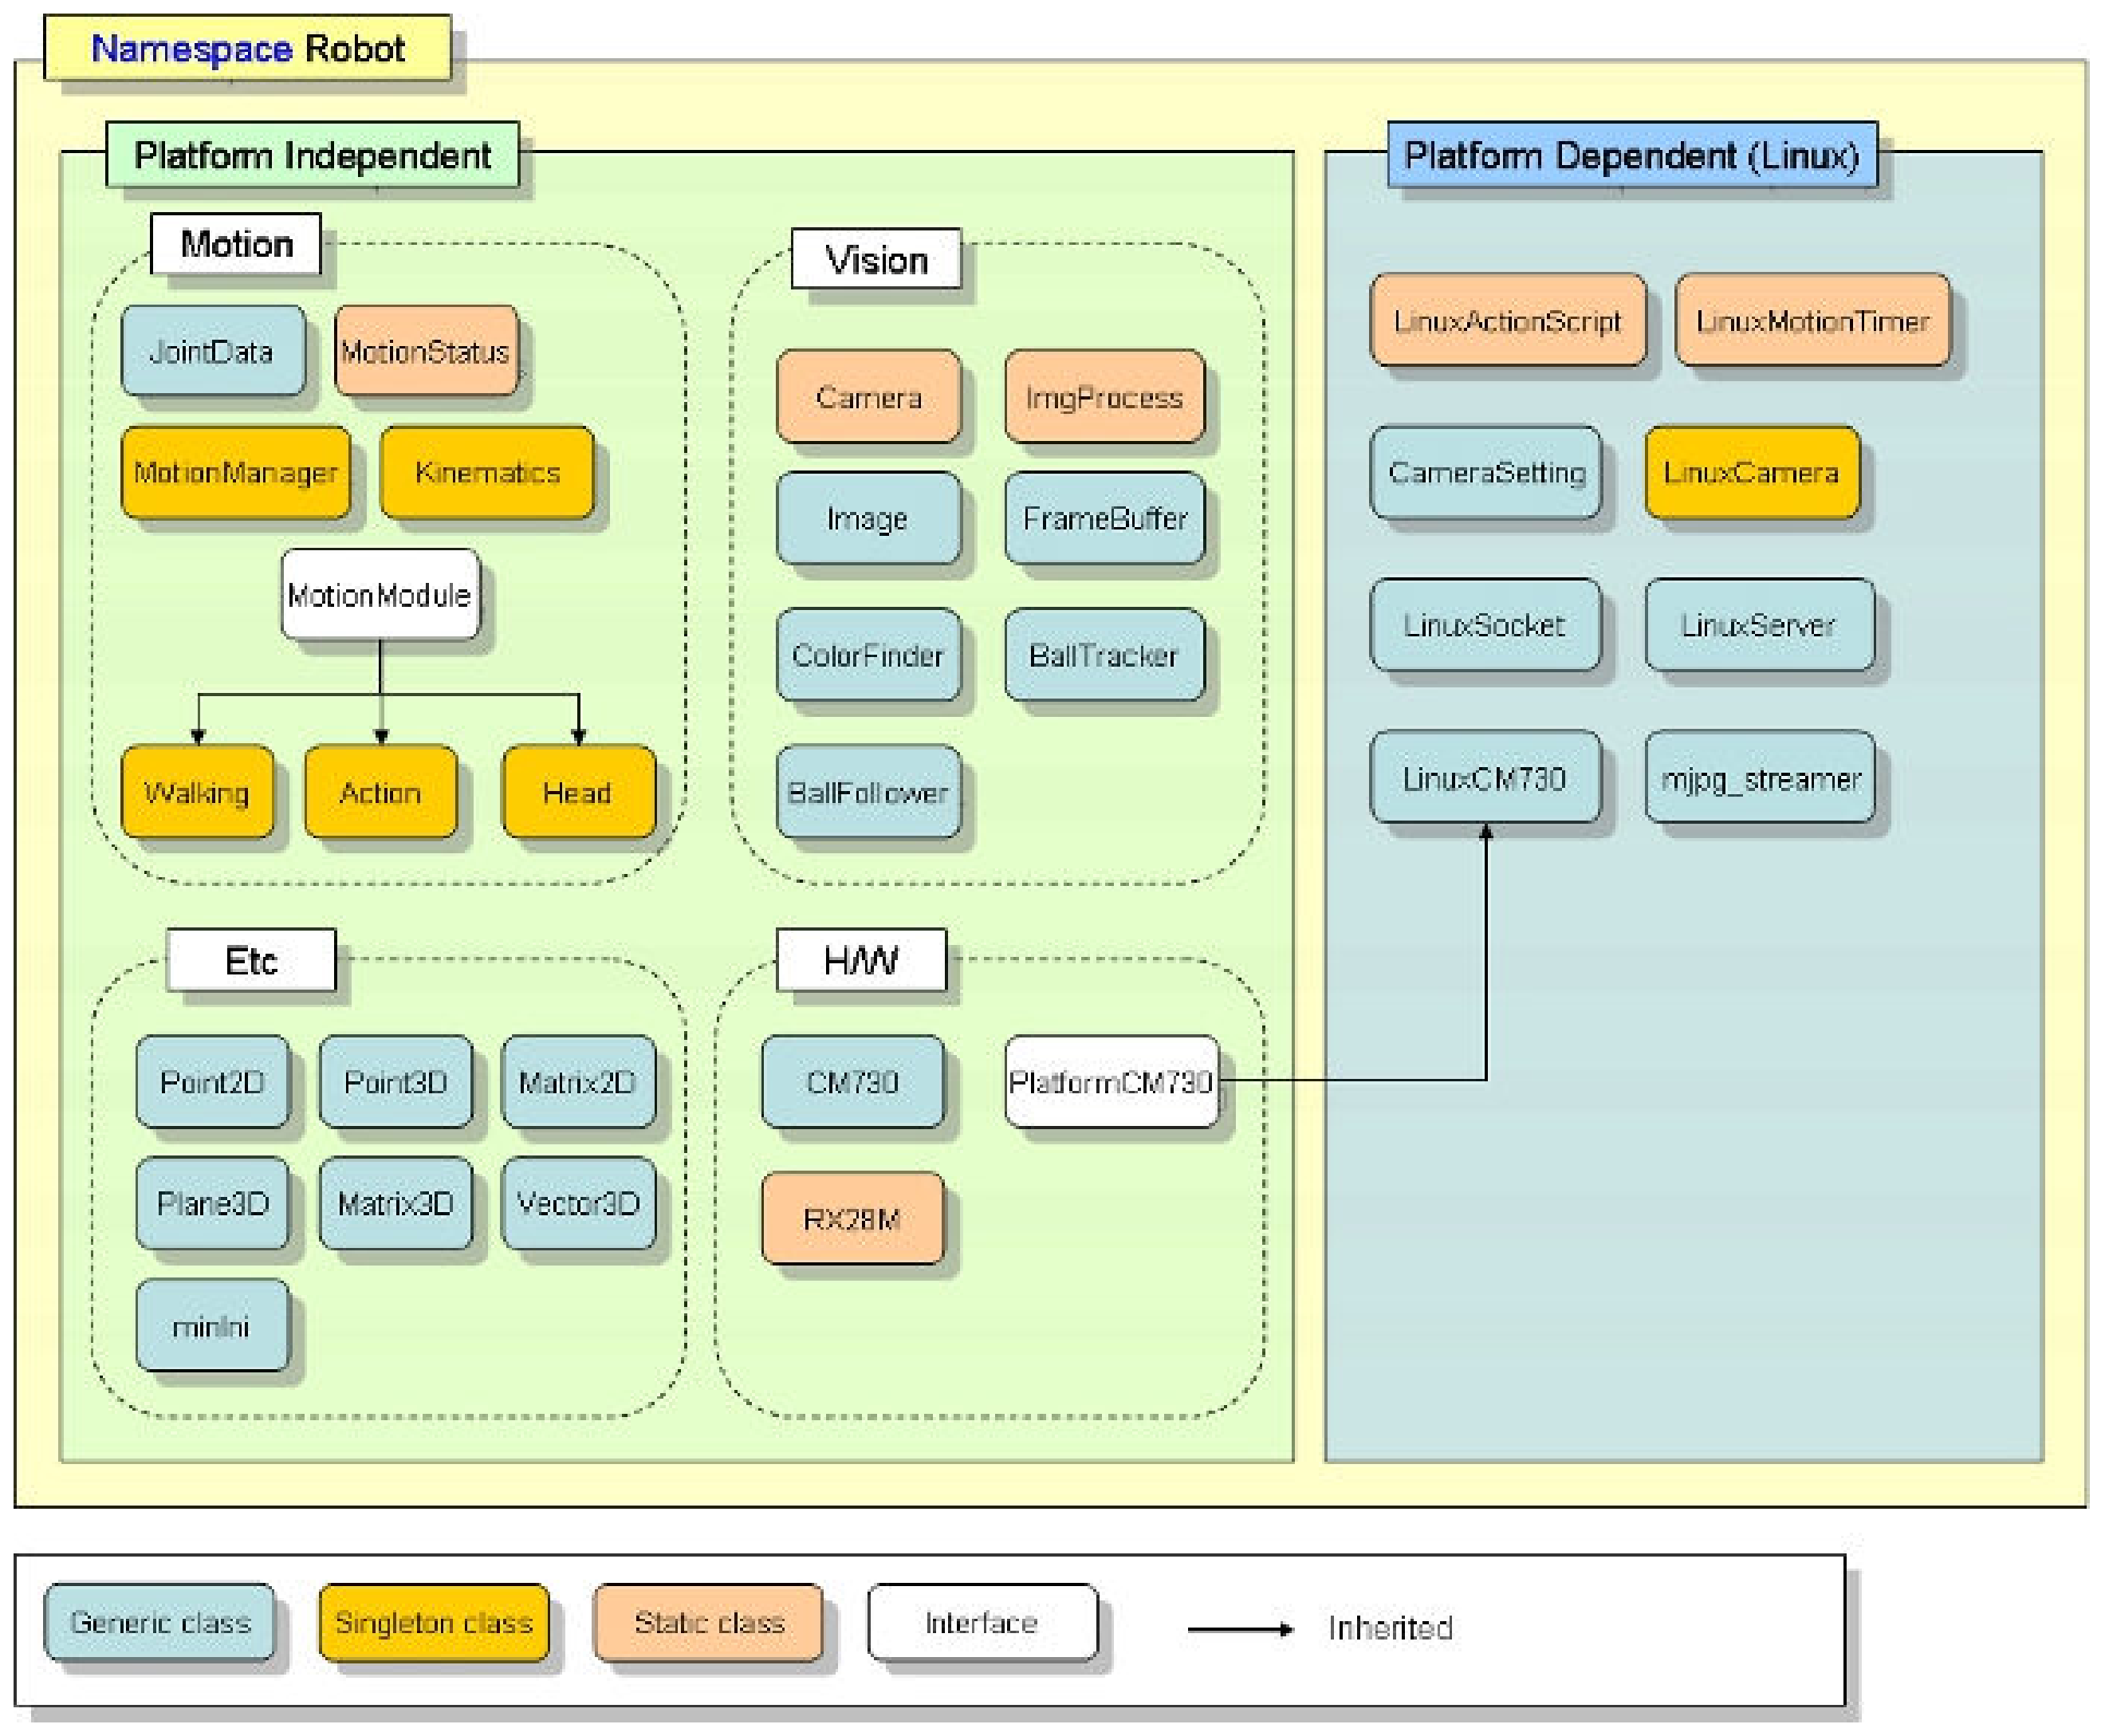
\includegraphics[width=1\linewidth]{1_framework_class_diagram}}
\caption{Диаграмма классов DARwIn Framework.}
\label{im:1_framework_class_diagram}
\end{figure}

Все классы находятся в области видимости Robot и делятся на платформонезависимые элементы и элементы, написанные для операционной системы Linux. Сам робот работает под управлением операционной системы Linux Ubuntu 9.10. Из данных классов нас будут интересовать елементы групп H/W и Motion.

Класс CM730 отвечает за взаимодействие программы-контроллера с субконтроллером робота. Он предоставляет возможность получать информацию с устройств, подключенных к данной плате (гироскоп, акселерометр, кнопки, сервоприводы и т.д.), а так же отправлять данные на светодиодные индикаторы и сервоприводы. Отправка и получение данных с соответствующих устройств происходит с задержкой в 6 мс. Для увеличения производительности отправка и получение данных на все моторы робота происходит единым пакетом данных.

Для управления движениями робота была реализованна группа классов Motion. Класс JointData является контейнером данных для взаимодействия с моторами робота. Он хранит PID данные и позиции для каждого сервопривода, а так же предоставляет публичные методы для взаимодействия с этими переменными.

Класс Kinematics имеет статические поля с информацией о длинах состовляющих ноги робота (высота бедра, голени и стопы) и информация о позиции камеры. Информации о длинах состовляющих рук в данном классе отсутствуют и дальнейшем будут взяты из документации о кинематике робота. % TODO Ссылка на документацию

MotionModule является интерфейсом для управления движениями робота. Данный интерфейс хранит экземпляр JointData для взаимодействия алгоритма с моторами. Производитель робота предоставляет в данном фреймворке готовый модуль управления походкой робота (Walking), модуль вопроизведения записанных движений (Action) и модуль для управления головой робота (Head).

Подробнее стоит рассмотреть реализацию модуля походки робота. Параметры походки читаются из конфигурационного *.ini файла с помощью библиотеки miniIni, которая идет в комплекте с данным фреймворком. Далее приведены основные параметры, которые описываются в файле: начальное смещение стопы по оси X в миллиметрах, начальное смещение стопы по оси Y в миллиметрах, начальное смещение стопы по оси Z в миллиметрах, начальный разворот стопы стопы вокруг оси X в градусах, начальный разворот стопы стопы вокруг оси Y в градусах, начальный разворот стопы стопы вокруг оси Z в градусах, угол наклона туловища в градусах, период двух шагов в миллисекундах, соотношение времени между периодом переноса ноги и остановки, длина шага в миллиметрах, максимальная амплитуда поднятия стопы в миллиметрах, амплитуда смещения туловища влево-вправо в миллиметрах, амплитуда подъема-опускания туловища в миллиметрах. Данный перечень параметров можно сгруппировать в параметры положения и вращения туловища и параметры положения и вращения левой и правой стопы, что пригодится в дальнейшем при разработке системы управления роботом. Сам алгоритм походки состоит и поочередного переноса стопы по синусоидальной траектории: высчитывается позиция стопы в каждый момент времени и решается задача обратной кинематики для расчета позиций моторов. Так же стоит обратить внимание, что алгоритм реализован некорректно при развороте стопы вокруг оси Z и ненулевом наклоне туловища: наклон робота происходит путем добавления угла наклона к позиции моторов бедер, а при вращении ноги вокруг оси Z данный угол должен был распределяться на два мотора на каждой ноге. В разработке системы управления механикой этот фактор так же будет учтен.

Статический класс MotionStatus является контейнером для данных, полученных с гироскопа, акселерометра и кнопок робота.

Класс MotionManager является связующим звеном между реализациями MotionModule и MotionStatus с классом CM730: класс передает данные из активных модулей движения непосредственно на физические моторы.
Для демонстрации взаимодействия классов ниже приведена схема передачи данных между модулями робота (Рис. \ref{im:1_framework_pipeline}), приведенная в официальной документации робота.

\begin{figure}[h]
\center{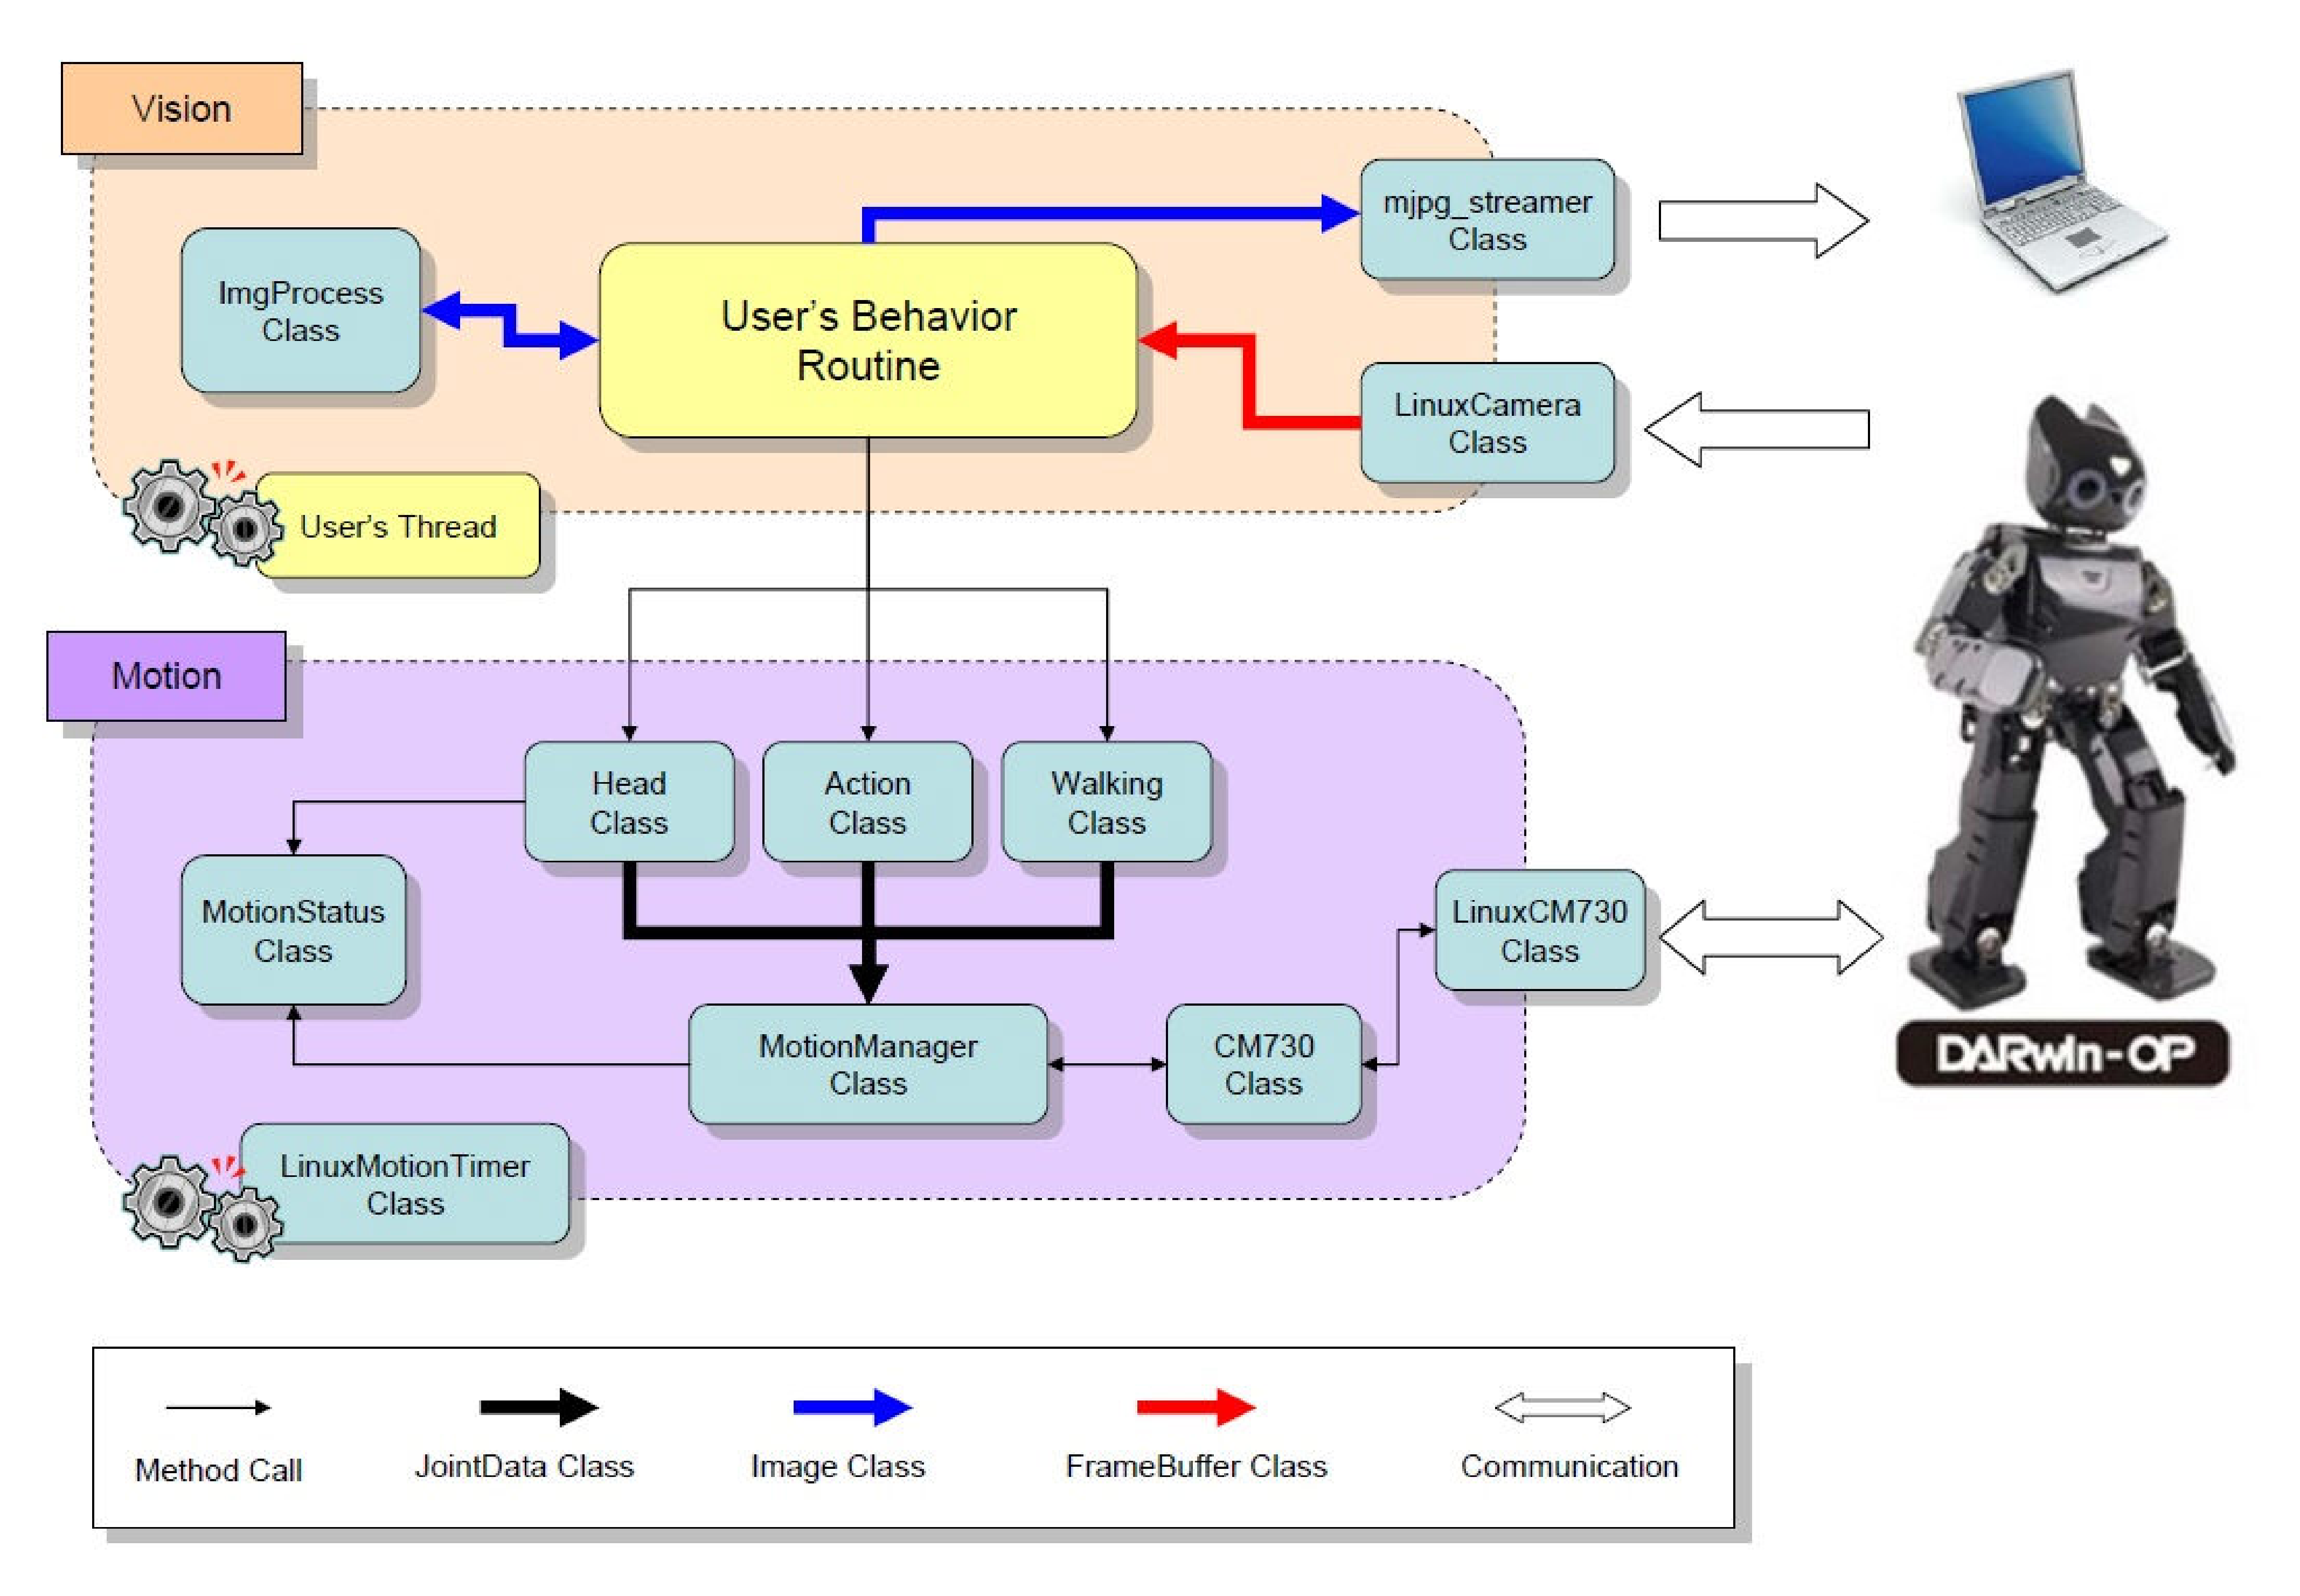
\includegraphics[width=1\linewidth]{1_framework_pipeline}}
\caption{Диаграмма передачи данных между модулями робота.}
\label{im:1_framework_pipeline}
\end{figure}

Обобщив выше сказанное можно заметить, что в интерфейсе программирования роботом отсутствует готовая реализация механизма программным управлением движений с помощью перемещений декартовой системы координат. Исходя из этого можно утверждать, что, например, при игре в футбол возможности удара по мячу у данного робота ограничивается механизмом воспроизведения записанных движений и отсутствует возможность расчета траектории удара. 

\section{Анализ симуляционной среды Webots}

Для возможности программно симулировать поведение робота был выбран кросплатформенный робототехнический симулятор Webots 8.0. В данном симуляторе имеется полная поддержка DARwIn-OP, за исключением возможности воспроизведения звука. Так же симулятор позволяет запускать и тестировать код непосредственно на самом роботе.

В данном разделе будут рассматриваться исключительно аспекты программного управления роботом DARwIn-OP. Это требуется для получения представления о том, как организовать поддержку симулятора при разработке библиотеки управления механикой роботом. Обзор всех возможностей симулятора для данного робота выходит за пределы данной работы.

Перед тем, как начать рассмотрение базовых классов, предоставляемых симулятором для взаимодейставия роботом, стоит упомянут о различии процесса сборки контроллера (программы управления роботом) под симулятор и для компиляции контроллера на реальном роботе. Симулятор Webots предоставляет разработчику набор абстрактных классов для взаимодействия с роботом. Компиляция для запуска программы на физической модели робота происходит с ключом -DCROSSCOMPILATION для компилятора gcc. Другими словами этот ключ объявляет макрос C/C++ при сборке всего исходного кода. С помощью механизма макроподстановки в языке данный ключ сообщает о том, нужно ли использовать механизмы управления, предоставляемые Darwin Framework, или контроллер будет использовать классы для поддержки симуляции в среде Webots. Контроллер, собранный с поддержкой симуляции, нельзя напустить на роботе как и наоборот.

Далее приведено описание базового набора классов для управления роботом. При компиляции контроллера для запуска на роботе перечисленные все классы являются оберткой вокруг вызовов методов классов Darwin Framework.

Ключевым классом контроллера является класс Robot. Класс пользовательского контроллера обязательно должен быть наследован от данного класса. В нем происходит инициализация оборудования и основных механизмов, а так же происходит обновление данных устройств. Для робота заданы хэш-таблицы с существущим набором светодиодных индикаторов, сервоприводов, позиционных сенсоров, гироскопа, акселерометра и кнопок. Для поддержки пошаговой симуляции в классе определен метод int step(time\_step). Данный метод должен вызываться на каждой итерации работы контроллера для обновления данных и взаимодействия с симулятором.

Класс Accelerometer отвечает за работу акселерометра. Класс возвращает целочисленное значение от 0 до 1024, что является соответственно диапазону значений от $-3g$ до $3g$.

Класс Gyro отвечает за работу гироскопа. Класс возвращает целочисленное значение от 0 до 1024, что является соответственно диапазону значений от -160 град/сек до 160 град/сек.

Для взаимодействия с сервоприводами в симуляционной среде существуют два класса: PositionSensor и Motor. Первый класс получает данные о текущем положении двигателя, а второй - для установки значений на привод. Для каждого двигателя программно задано максимальное и минимальное значение угла поворота. Классы предоставляют большой набор методов для взаимодействия с моторами. Листинг данных методов приведен ниже:

\lstset{language=C++}
\begin{lstlisting}
void enablePosition(int ms);
void disablePosition();
void enableMotorForceFeedback(int ms);
void disableMotorForceFeedback();
int getSamplingPeriod();
int getType() const;
void setVelocity(double vel);
void setForce(double force);
void setMotorForce(double motor_force);
void setControlP(double p);
void setPosition(double position);
void setAcceleration(double force);
double getMotorForceFeedback() const;
double getPosition() const;
double getTargetPosition();
double getMinPosition();
double getMaxPosition();
\end{lstlisting}

Так же стоит упомянуть о том, что для управления приводами на реальном роботе стоит использовать MotionModule из Darwin Framework вместо класса Motor. Это связано с тем, что отправка значений на реальные сервоприводы происходит в большой задержкой в случае с классом Motor. Данное наблюдение было обнаружено экспериментальным путем и нигде ранее в официальных источниках не было документированно.

Так же для данного робота предоставляются три класса менеджеров: DARwInOPGaitManager, DARwInOPMotionManager и DARwInOPVisionManager. Последний класс из данного списка отвечает за обнаружение объектов на изображении с камеры и в рамках данной работы он не представляет особого интереса. DARwInOPMotionManager является фасадом между Webots и классом Action из Darwin Framework. Данный модуль позволяет воспроизводить заранее записанный набор движений, хранящиеся во внешнем фаиле.

Подробнее будет рассмотрен класс DARwInOPGaitManager. По аналогии с классом DARwInOPMotionManager данный менеджер является оберткой вокруг класса Walking из Darwin Framework. Конструктор данного класса принимает одним из обязательных аргументов указатель на экземпляр класса Robot, описанного ранее в данном разделе. Это требуется для получения экземпляров класса Motor для возможности симуляции работы алгоритма менеджера в Webots. В случае отсуствия макроса CROSSCOMPILATION используется класс Walking для вычисления значений моторов и эти данные передаются экземплярам класса Motor. В случае компиляции алгоритма для запуска на роботе все позиции моторов будут прочитаны из класса JointData в экземпляре класса Walking с помощью MotionManager и через CM730 данные будут переданы на сервоприводы робота. Так же конструктор принимает \*.ini файл для настройки параметров походки, которые быле описаны в предыдущем разделе. В классе присутствуют методы $enable()$ и $disable()$, которые соответственно активируют и дезактивируют MotionManager из Darwin Framework. Так же имеются методы для задания скорости движения по оси $x$, по оси $y$ и угловая скорость $\alpha$

На основе структуры класса DARwInOPGaitManager разработан класс-фасад для поддержки симуляции разработанной библиотеки управления сервоприводами робота. Данное разделение классов требуется для возможности запуска системы управления без подключения классов симулятора.

Ниже приведен снимок экрана для демонстрации интерфейса симулятора Webots (Рис. \ref{im:1_webots_sample_window}). Симулятор был запущен на операционной системе ArchLinux с графическим пользовательским интерфейсом GNOME 3. На других операционных системах и графических окружениях работа симулятора не тестировалась. Это связано с тем, что одни из самых популярных на сегодняшний день реализации гуманоидных роботов (Nao и Darwin) находятся под управлением различных дистрибутивов операционной системы Linux и в рамках данной работы поддержка других платформ не ставилась в цели работы.

\begin{figure}[h]
\center{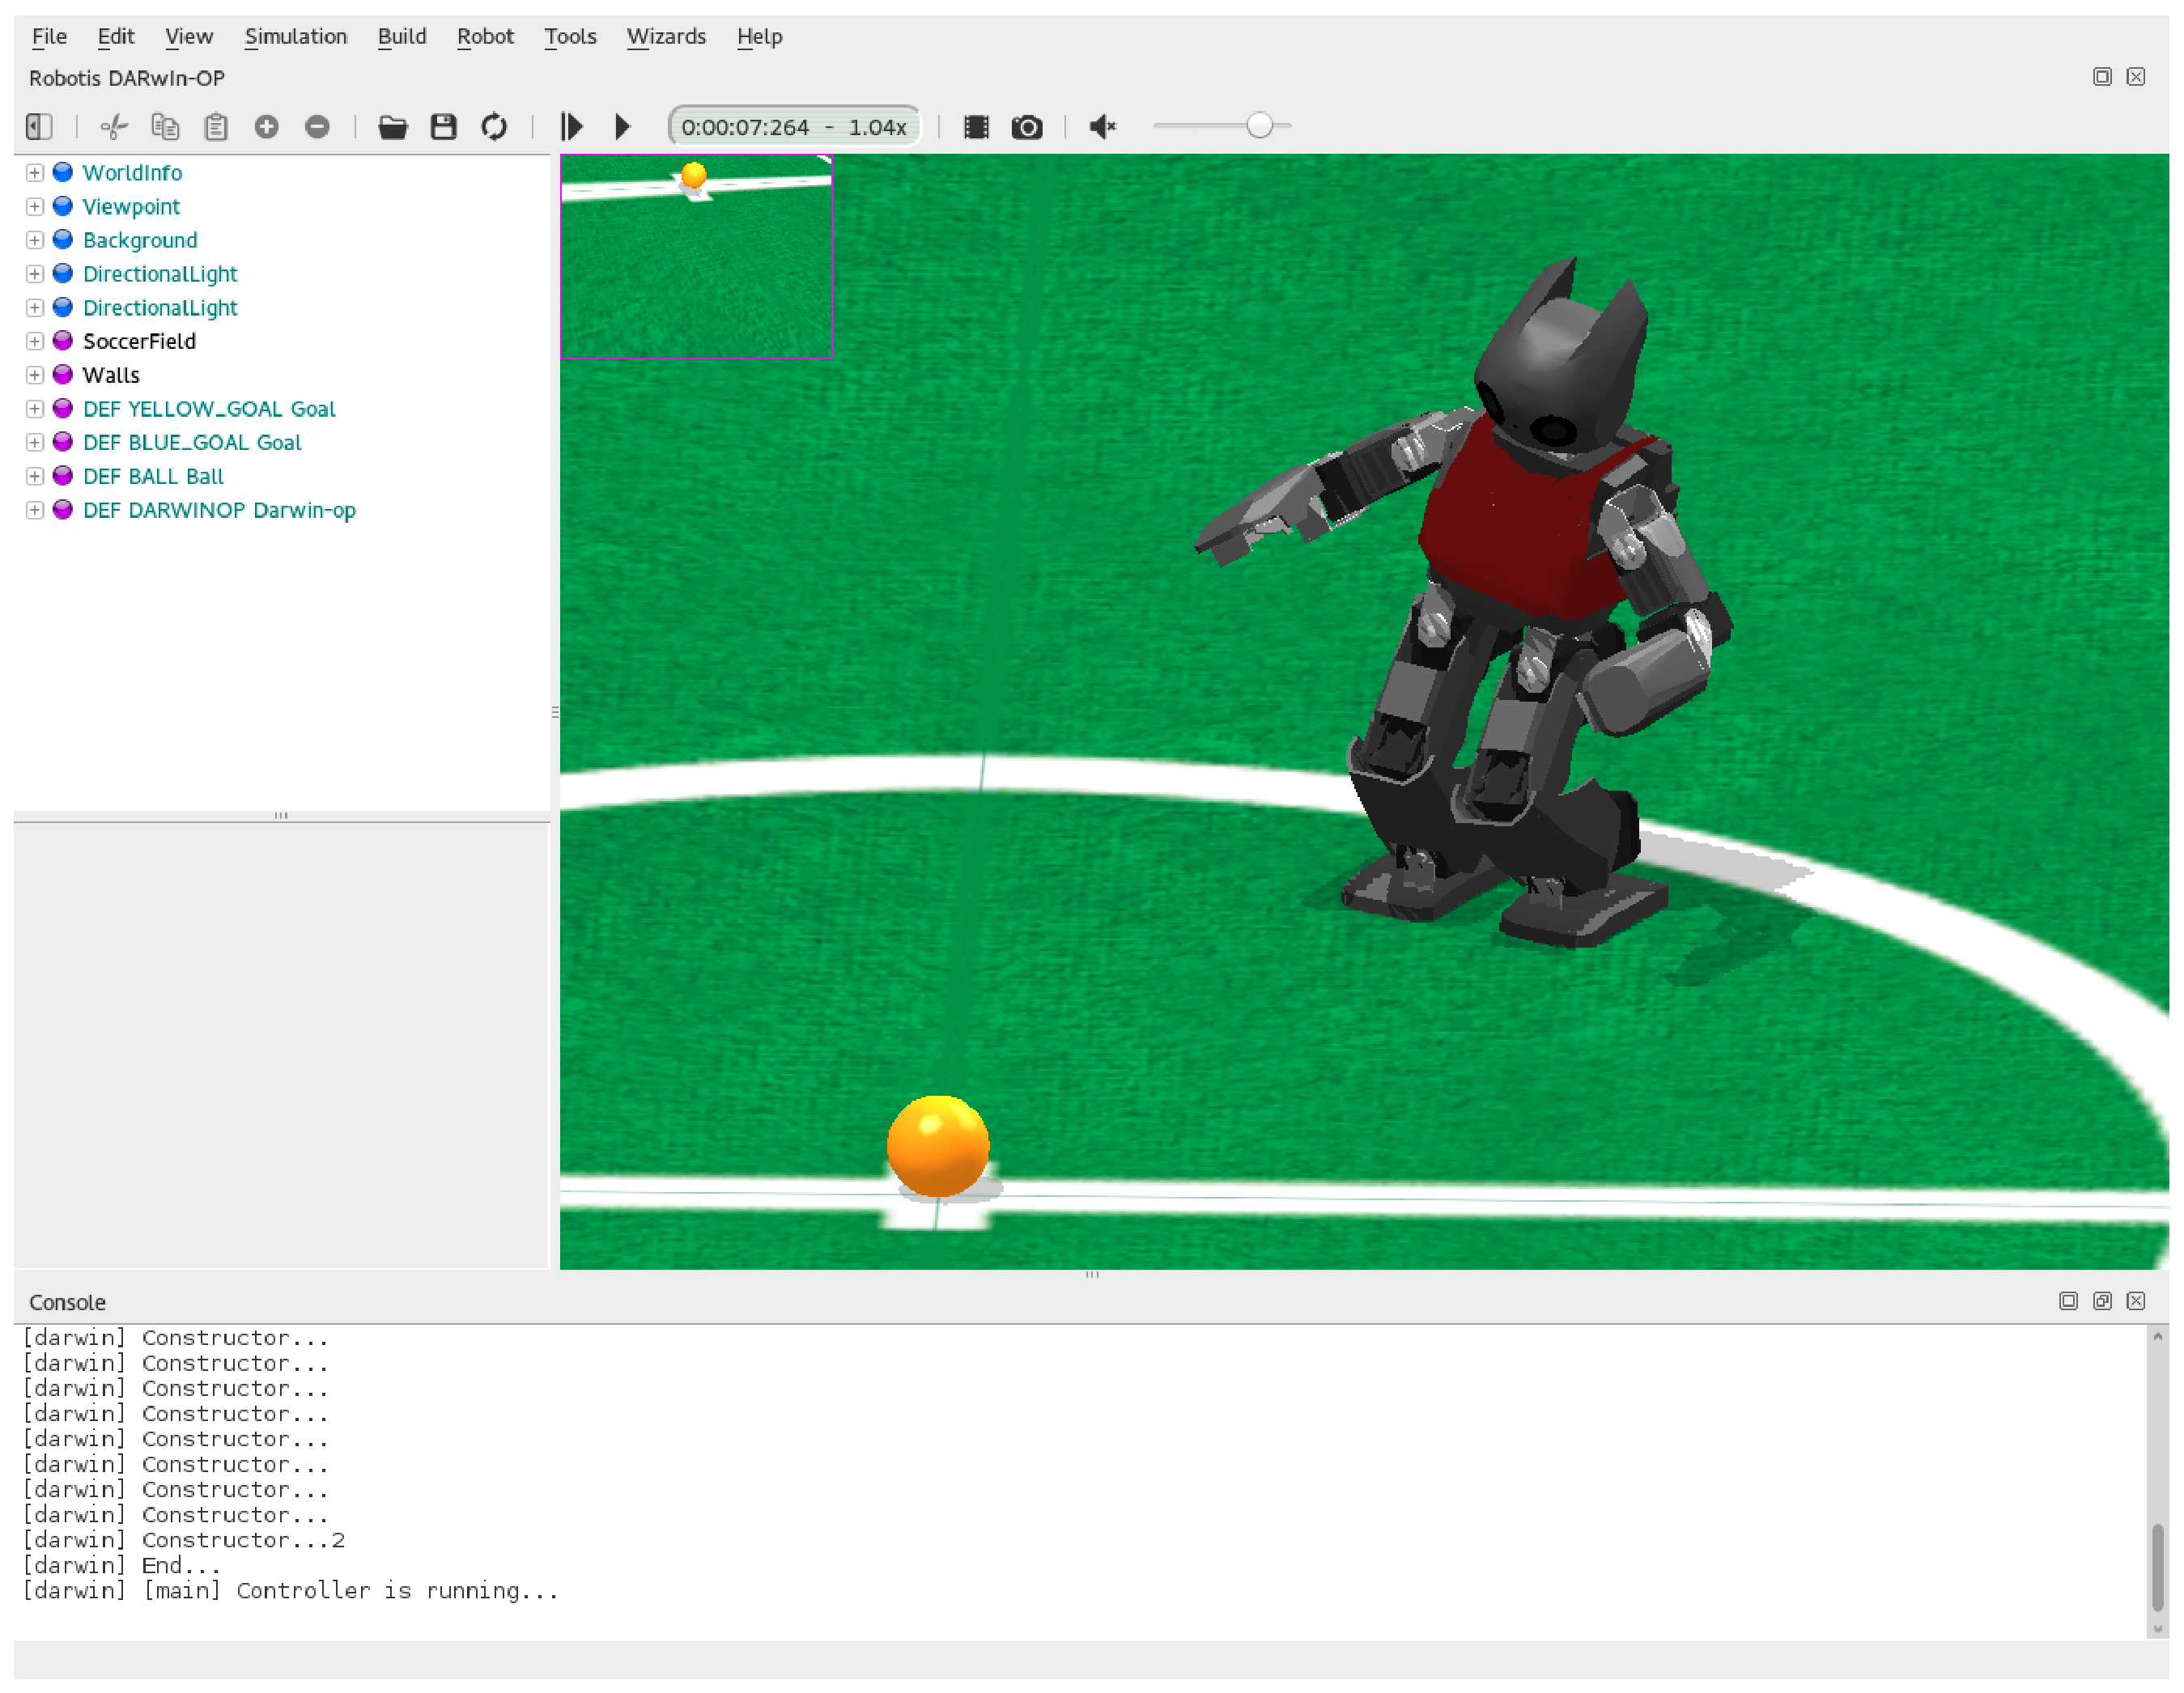
\includegraphics[width=1\linewidth]{1_webots_sample_window}}
\caption{Окно симулятора Webots.}
\label{im:1_webots_sample_window}
\end{figure}

Для запуска пользовательского контроллера на симулируемой модели робота требуется заранее произвести компиляцию программы с помощью Makefile и утилиты make. Образец Makefile был взят из демонстрационного контроллера Soccer. Так же каждый отдельный контроллер должен находиться в отдельном каталоге. Это требуется для того, чтоьбы симулятор мог найти битарные файлы контроллера. Название каталога должно соответствовать названию бинарного файла. Выбрать контроллер можно с помощью соответственного пункта в меню (слева в окне симуляции) у объекта "DEF DARWINOP Darwin-OP".

Так же симулятор позволяет добавлять другие экземпляры робота на отображаемую сцену и запускать на нем отдельные требуемые реализации контроллера. Это позволят проводить тестирование поведения на одновременно на нескольких роботах.

В Webots была замечена недокументированная особенность в поведении перенаправления данных со стандартного потока вывода в консоль симулятора. Данная консоль перенаправляен данные, полученные со стандартного потока вывода работающего контроллера. Отображение данных происходит только после получения символа конца строки (ASCII код соответствует значению 0A в шестнадцатиричной системе счисления). Другими словами выведенная строка не будет отображена без символа конца строки.

Для отладки исходного кода имеется возможность использовать утилиту gdb. Для поддержки отладки требуется добавить флаг $-g$ при запуске компилятора gcc. Для этого достатачно в Makefile требуемого контроллера написать следующие строки:

\lstset{language=[gnu] make}
\begin{lstlisting}
CFLAGS = -g
\end{lstlisting}

Данная строка добавит соответствующий флаг компиляции и будет использован в Makefile, который 

Для подключения утилиты отладки требуется в системной командной строке произвести запуск gdb и выполнить команду attach к PID (идентификатор процесса) запущенного контроллера. Идентификатор процесса можно получить из утилиты gnome-system-monitor или из другого подобного приложения. Подробно рассматриваться процесс отладки в данной работе не будет. Более полную информацию можно получить из официальной документации утилиты gdb.

Так же симулятор позволяет запускать контроллер для Darwin-op на реальной модели робота (Рис. \ref{im:1_webots_transfer}) и получать информацию с устройств робота (Рис. \ref{im:1_webots_position_sensors}).

\begin{figure}[h]
\center{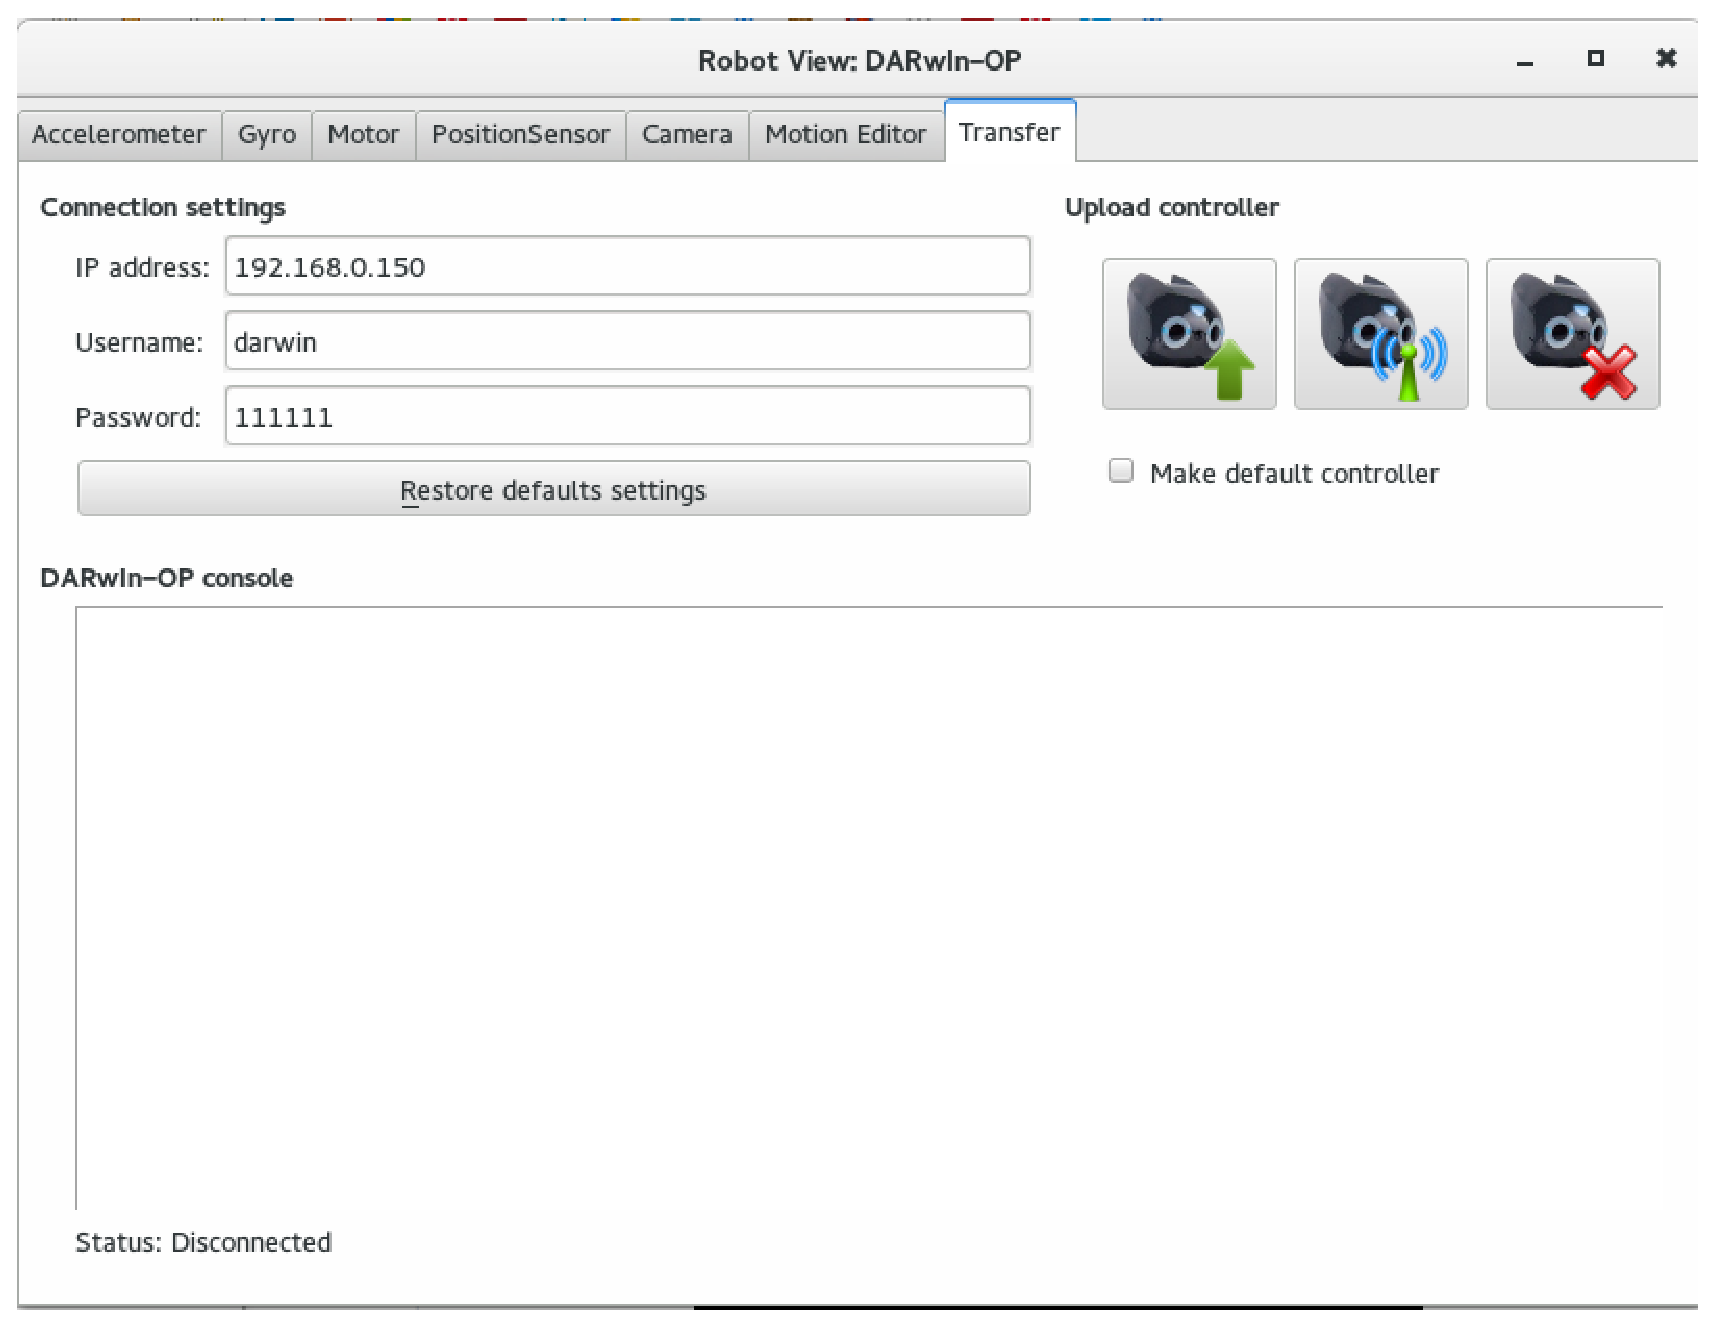
\includegraphics[width=0.5\linewidth]{1_webots_transfer}}
\caption{Окно запуска контроллера на реальном роботе.}
\label{im:1_webots_transfer}
\end{figure}

Подключение к роботу происходит по ssh протоколу. При первом подключении симулятора к реальному роботу происходит копирование исходного кода контроллера и библиотек Webots в соответствующий во внутренний диск на роботе и далее происходит компиляция требуемых компонентов. Данные о процессе сборки выводятся в консоль. При успешном завершении процесса сборки требуемый контроллер сразу же запускается на роботе. Если контроллер не был запущен, то данный процес должен выполнен вручную через ssh соединение вне симулятора. Причина, по контроллер не исполняется автоматически, установлена не была.

\begin{figure}[h]
\center{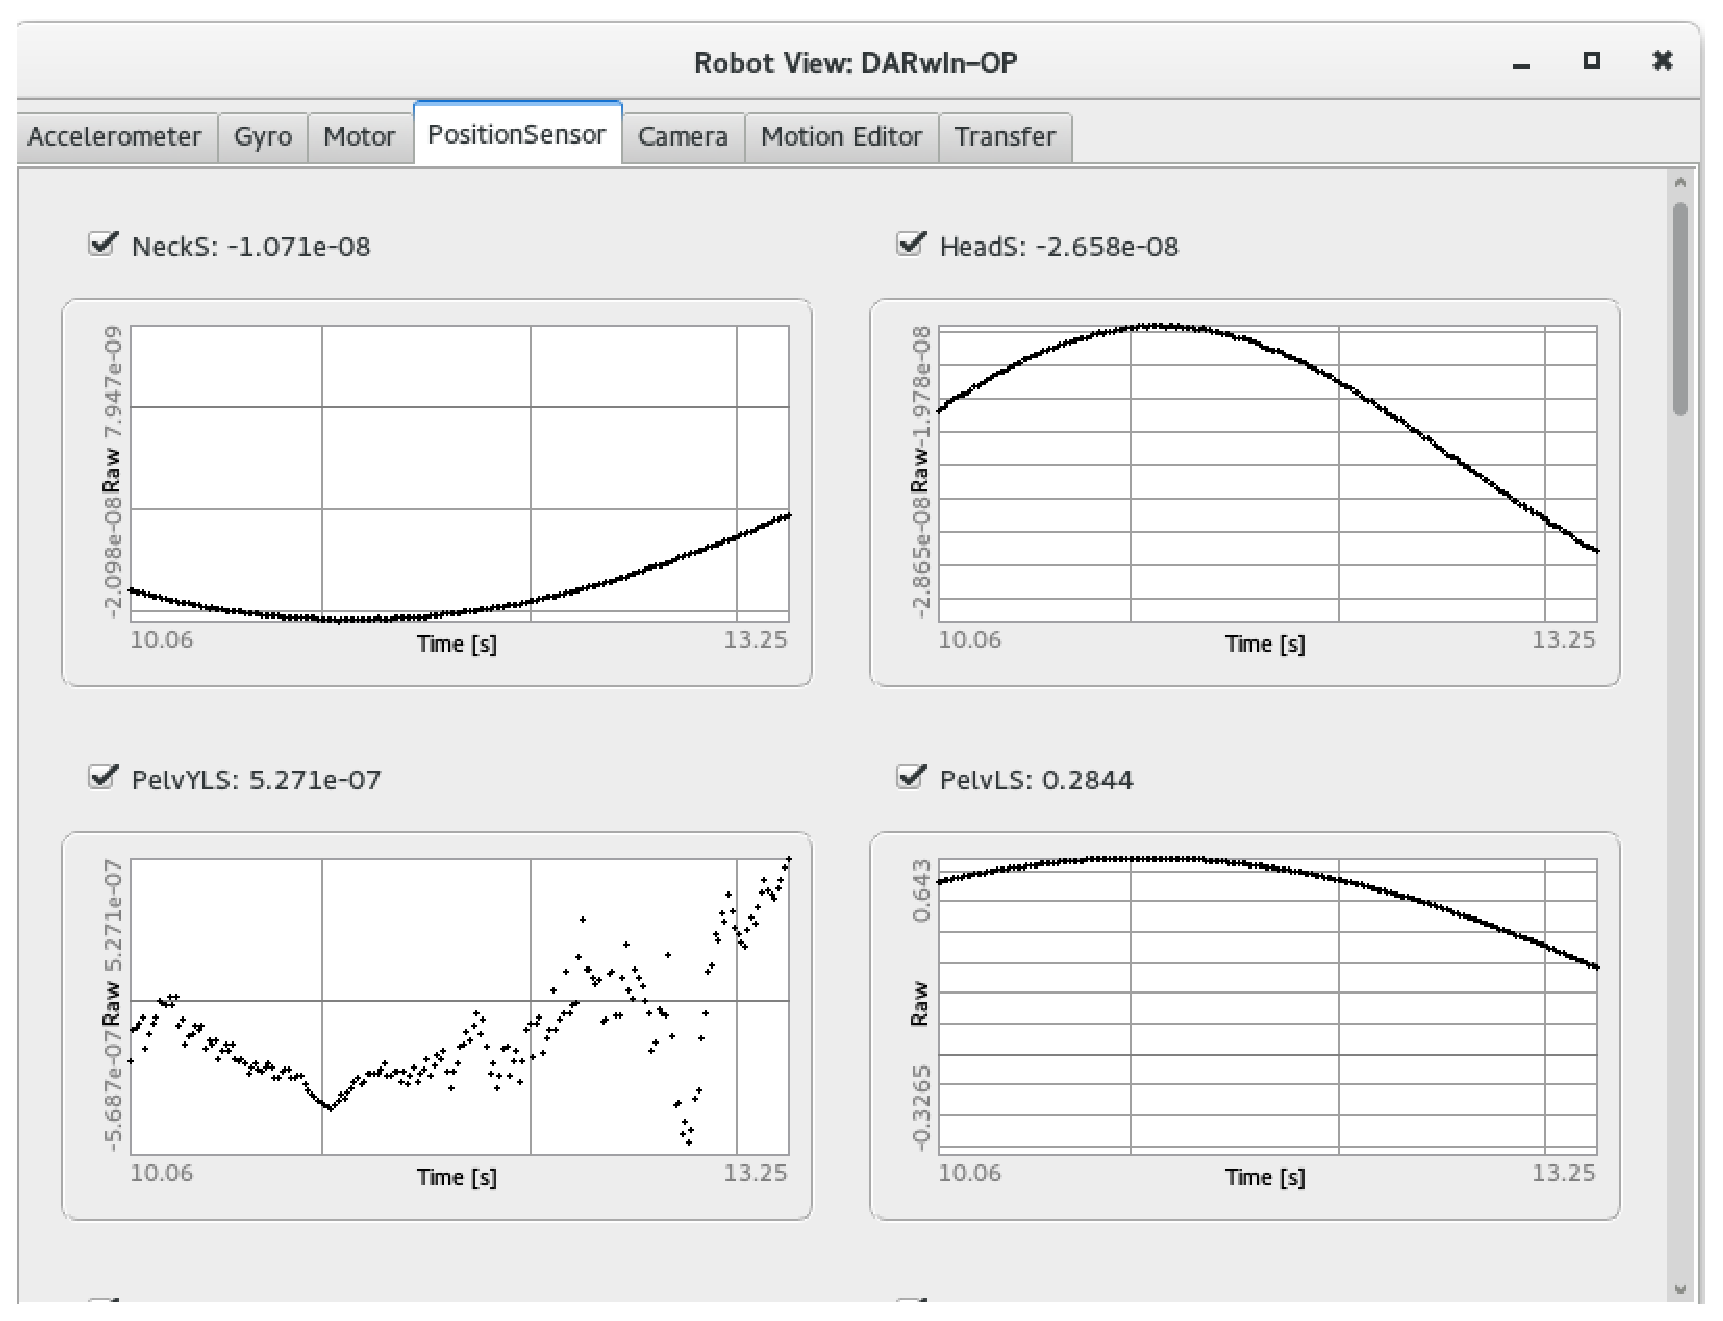
\includegraphics[width=0.5\linewidth]{1_webots_position_sensors}}
\caption{Показания позиционных сенсоров при выполнении движения.}
\label{im:1_webots_position_sensors}
\end{figure}

Для возможности компиляции проекта, исходный код которого находится в разных подкаталогах, требуется внести некоторые изменения в Makefile на роботе, который находится в родительском каталоге директории с исходным кодом. Подробнее об этом будет сказано позже. Стоит заметить, что данный файл нужно редактировать после компиляции основных компонентов Webots на роботе, так как симулятор копирует данный файл из неизвестного источника при первом запуске на роботе. Данный факт был обнаружен экспериментальным путем и ранее никак не документирован.

\section{Анализ NAO SDK}

В данном разделе проведен беглый обзор компонента управления сервоприводами робота из NAO SDK. В данном компоненте имеются некоторые ключевые особенности, которые позволят разработать интерфейс класса управления механикой для Darwin-OP.

